\section{Experiment}
\iffalse
https://github.com/HAIRLAB/Pre_Surv_COVID_19/

The choice of the cell is usually guided by the task at hand [J. Chung, C. Gulcehre, K. Cho, and Y. Bengio. Empirical evaluation of gated recurrent neural networks on sequence modeling.].
In all experiments we use an AE with 3 hidden layers, { D x , 30, D z , 30, D x } ; the number of neurons in the intermediate layers (30) has been set after preliminary experiments and is not a critical hyperparameter (comparable results were obtained using 20 or 40 neurons).
% In each experiment, we train the models for 5000 epochs with mini-batches containing 32 MTS using the Adam optimizer [kingma2014adam, D. Kingma and J. Ba. Adam: A method for stochastic optimization.] with an initial learning rate of 0.001.
% Data are in random order
% We consider the problem of classifying patients with and without surgical site infections from their blood samples.
% However, an important question for any autoencoder-style model is what prevents it from learning an identity mapping and effectively copying the input to the output. In that case all the information about the input would still be present but the representation will be no better than the input. There are two factors that control this behaviour. First, the fact that there are only a fixed number of hidden units makes it unlikely that the model can learn trivial mappings for arbitrary length input sequences.
% For this purpose, machine learning tools selected three biomarkers that predict the mortality of individual patients more than 10 days in advance with more than 90\% accuracy:

The problem was formulated as a classification task, where the inputs included basic information, symptoms, blood samples and the results of laboratory tests, including liver function, kidney function, coagulation function, electrolytes and inflammatory factors, taken from originally general, severe and critical patients (Table 1), as well as their associated outcomes corresponding to either survival or death at the end of the examination period. 
Medical records were collected by using standard case report forms that included epidemiological, demographic, clinical, laboratory and mortality outcome information (Table 2 and Supplementary Data 1).
The clinical outcomes were followed up to 24 February 2020.
% The medical information of all patients collected between 10 January and 18 February 2020 were used for model development.
Of the 375 cases included in the subsequent analysis, 201 recovered from COVID-19 and were discharged from the hospital, while the remaining 174 died> deceased.
% The performance models were evaluated by assessing the classification accuracy (ratio of true predictions over all predictions), the precision, sensitivity/recall and F1 scores (defined below): Definition of metrics with TP FP TN FN.

Selecting how deeper the model should be is another aspect of hyperparameter optimisation which can generally go from a single layer to three to four-layer deep model architecture where a three-layer architecture is used mostly in complex learning tasks. 

Because of the rapid spread of the virus, there has been a sharp increase in the demand for medical resources required to support infected people. Despite the desperate efforts to contain the disease and slow down its spread, many countries have been suffering from the shortage of hospital beds and critical care equipment for the timely treatment of ill patients[Ranney, M. L., Griffeth, V. & Jha, A. K. Critical supply shortages—The need for ventilators and personal protective equipment during the Covid-19 pandemic.,Gondi, S. et al. Personal protective equipment needs in the USA during the COVID-19 pandemic., Smereka, J. & Szarpak, L. The use of personal protective equipment in the COVID-19 pandemic era.]. Therefore, in addition to efficient diagnosis and treatment, accurate prognosis prediction is necessary to reduce the strain on healthcare systems and provide the best possible care for patients. When allocating limited medical resources, prediction models that estimate the risk of a poor outcome in an infected individual based on pre-diagnosis information could help to effectively triage patients.

In order to study the important blood biomarkers for predicting disease mortality, a retrospective study was conducted on 375 COVID- 19 positive patients admitted to Tongji Hospital (China) from January 10 to February 18, 2020. Demographic and clinical characteristics, and patient outcomes were investigated using machine learning tools to identify key biomarkers to predict the mortality of individual patient. A nomogram was developed for predicting the mortality risk among COVID-19 patients.

Yan et al. [21] reported a machine learning approach to select three biomarkers (lactic dehydrogenase (LDH), lymphocyte and high-sensitivity C-reactive protein (hs-CRP)) and using them to predict individual patients mortality, 10 days ahead with more than 90 percent accuracy. 
Blood samples collected between 10 January and 18 February, 2020 from 375 patients in Wuhan, China were retrospectively analyzed to identify reliable and relevant markers of mortality risk. Medical records were collected using standard case report forms, which included information on epidemiological, demographic, clinical, laboratory and mortality outcomes. Yan et al. [21] has published the dataset along with the article and the original study was approved by the Tongji Hospital Ethics Committee. Patients’ exclusion criteria for the study were: Age (<18 years), pregnant, breast- feeding and missing data (>20\%). Out of 375 patients, 187 (49.9\%) had fever while cough, fatigue, dyspnea, chest distress and muscular soreness were present in 52 (13.9\%), 14 (3.7\%), 8 (2.1\%), 7 (1.9\%) and 2 (0.5\%) patients respectively.
Of the 375 patients, 174 (46.4\) died, while 201 (53.6\%) patients recovered from COVID-19 and were discharged from hospital. Figure 1 summarizes the outcome of patients based on their initial conditions: general (197), severe (27) and critical (151). The minimal, maximal and median follow-up times (from hospital admission to death or discharge) for all 375 patients are 0 days, 35 days and 12 days, respectively.
Table 1 summarizes the demographic characteristics, clinical characteristics, and clinical outcomes of the subjects in the death and survival groups. There were 142 (37.9\%) patients, who were Wuhan residents, 2 (0.5\%) had contact with confirmed or suspected patients, 24 (6.4\%) were from familial cluster, 7 (1.9\%) were health workers, 2 (0.5\%) had contact with Huanan Seafood Market and 198 (52.5\%) had no contact history.

The main problem of neural networks, and therefore also of LSTMs, is the fact that is not always easy to understand how the network can identify the relationship between the input data and the target class.
\fi
%%%%%%%%%%%%%%%%%%%%%%%%%%%%%%%%%%%%%%%%%%%%%%%%%%%%%%%%%%%%%%%%%%%%%%%%%%%%%%%%%%%
%% Precision and Recall on what? on survival and death both?
% [We design experiments to accomplish the following objectives:]
% Experiment section is organized as follows:
% 1. Prediction Performance on Classification on mortality.
% 2. blah.
% Convergency graph where all k-th runs are in a single figure.

Our experiments consist of two parts; (1) we evaluate the prediction performance of the proposed model, and (2) we identify the biomarkers which are most predictive for mortality.

\subsection{Hyperparameters and Competing Models}
We use the following hyperparameters found by the grid search. For our semi-supervised autoencoder (SAE), the decoder $\phi_D$ has 3 fully connected layers with 200, 140, 100 nodes and hyperbolic tangent activation function except for the input layer and leaky Rectified Linear Unit (leaky ReLU, alpha = 0.1) for the input layer. Here we found that the leaky ReLU largely improves the reconstruction performance of decoder, as we presume that time stamp is the most important input feature for the decoder and this can be emphasized more with leaky ReLU activation function in a range $(- \infty, \infty)$, than the other activation functions in a smaller range. The predictor $\phi_P$ has 3 fully connected layers with 120, 60, 20 nodes and hyperbolic tangent activation function. The encoder $\phi_E$ has LSTM network with 60 units and hyperbolic tangent activation function. $\gamma_1$ and $\gamma_2$ in Eq.~\eqref{eq: objective} are set to 0.005 and 0.1. To minimize the loss function in Eq.~\eqref{eq: objective}, we use Adam optimizer~\cite{kingma2014adam} with learning rate of 0.0003 and the other parameters kept at their default values. We do not use any regularization or dropout technique, as they have not improved the performance. Considering our loss function is defined differently depending on the existence of label of sample, we train our model with the sample by sample instead of batch of samples. We build our model with Python 3.7 and Keras~\cite{chollet2015keras} framework. We use MacOS with 3.4 GHz Quad-Core Intel Core i5 CPU and 16 GB DDR4 Ram and it took 4 hours to train our model with 286 samples and 200 iterations.
% For prediction error, we have tried binary cross entropy and mean squared error, and mean squared error works better. Best Hyper-parameters are searched by following set of grid. Because RE\_DATE is important feature in decoder input, thus should be emphasized, we use leaky ReLU activation function at the input layer of decoder. And the prediction accuracy is improved with leaky ReLU at the input layer than tanh, while tanh works better in other layers.

For an ablation study to observe the effectiveness of our semi-supervised enrichment learning, we introduce supervised baseline LSTM (BLSTM) model as a competing model by removing decoders $\phi_{D}$ from our model SAE but with the same hyperparameters as our model. In addition to the longitudinal model, we use the following competitive models:
\begin{itemize}
    \item MLP with 5 fully connected layers of 200, 140, 100, 140, 200 nodes.
    \item Random Forest~\cite{ho1995random} (RF) with 34 max depth.
    \item Ridge Regression (RR) with regularization parameter of 1.0.
    \item Support Vector Machine (SVM) with regularization parameter of 1.0 and kernel function of radial basis function.
\end{itemize}
Since these competitive models are not longitudinal models, we provide the concatenation of most recent record $[\mathbf{x}_i^b, \mathbf{x}_i^{n_i}]$ to them. The training and test set both are provided to train SAE in a semi-supervised manner, while only the training set is provided to train the other competing models. Although the order of participants is randomly shuffled to avoid the bias, we use the same training and test data across all the competing methods for the fair comparison.

\subsection{Classification Performance}
%% Simple LSTM is ablation study.
We conduct the classification task to predict the mortality of COVID-19 patients more than 10 days in advance and evaluate the performance of the predictive models. The outputs of the models are rounded up to the binary. We evaluate the predictive models with the following metrics:
\begin{equation}
\begin{aligned}
    &\text{Accuracy} = \frac{TP + TN}{TP + TN + FP + FN},\\
    &\text{Precision} = \frac{TP}{TP + FP},\\
    &\text{Recall} = \frac{TP}{TP + FN},\\
    &\text{F}_1\text{-score} = 2 \times \frac{Precision \times Recall}{Precision + Recall}.
\end{aligned}
\end{equation}
In table~\ref{tab: experimetal results}, the average and standard deviation of the metrics across $k$ subgroups are reported following $k$-fold cross validation scheme. $k$ is set to 4 (the size of training set is 25\% or 75\% of the studied cohort) or 5 (the size of training set is 20\% or 80\% of the studied cohort).
% SAE, BLSTM, MLP, LASSO, RR, SVM denote the Semi-supervised BLSTM Auto Encoder (our model), Long Short Term Memory, Multi Layer Perceptron, Least Absolute Shrinkage and Selection Operator, Ridge Regression, Support Vector Machine, respectively.
% From the 75 dynamic features from blood samples, and 4 static features from patient's demographic, we predict the patient's mortality in 10 days.
\begin{table*}[h]
    % \footnotesize
    %\scriptsize
    % \small
    \setlength{\tabcolsep}{4pt} %% change column-wise separation.
    \centering
    \caption{The prediction performance of SAE and the competitive models from k-fold cross validation. The best prediction is denoted as bold font.}\label{tab: experimetal results}
    \begin{tabular}{|c|c|c|c|c|c|} %% 6 columns table
    \hline
    {\bfseries Test Set Size} & {\bfseries Model} & \multicolumn{1}{c}{{\bfseries Accuracy}} & \multicolumn{1}{c}{{\bfseries Precision}} & \multicolumn{1}{c}{{\bfseries Recall}} & {\bfseries $\text{F}_1$-score}\\ %% Headers
    \Xhline{1pt}
    \multirow{6}{*}{20\%} %% 6 rows group.
    & SAE & \multicolumn{1}{c}{{\bfseries 94.14$\pm$2.31}} & \multicolumn{1}{c}{\bfseries{93.35$\pm$2.45}} & \multicolumn{1}{c}{{\bfseries 93.15$\pm$2.84}} & {\bfseries 93.48$\pm$1.21}\\
    & BLSTM & \multicolumn{1}{c}{92.56$\pm$3.24} & \multicolumn{1}{c}{91.11$\pm$1.45} & \multicolumn{1}{c}{92.45$\pm$8.12} & 91.43$\pm$5.40\\
    & MLP & \multicolumn{1}{c}{80.63$\pm$11.52} & \multicolumn{1}{c}{76.58$\pm$10.94} & \multicolumn{1}{c}{83.80$\pm$11.97} & 80.02$\pm$11.14\\
    & RF & \multicolumn{1}{c}{83.25$\pm$11.89} & \multicolumn{1}{c}{78.03$\pm$11.15} & \multicolumn{1}{c}{88.77$\pm$12.68} & 83.05$\pm$11.86\\
    & RR & \multicolumn{1}{c}{79.32$\pm$11.33} & \multicolumn{1}{c}{76.76$\pm$10.97} & \multicolumn{1}{c}{79.54$\pm$11.36} & 78.12$\pm$11.16\\
    & SVM & \multicolumn{1}{c}{79.32$\pm$11.33} & \multicolumn{1}{c}{77.55$\pm$11.08} & \multicolumn{1}{c}{78.12$\pm$11.16} & 77.83$\pm$11.11\\
    \Xhline{1pt}
    \multirow{6}{*}{25\%} %% 6 rows group.
    & SAE & \multicolumn{1}{c}{{\bfseries 92.47$\pm$3.43}} & \multicolumn{1}{c}{{\bfseries 91.84$\pm$8.41}} & \multicolumn{1}{c}{{\bfseries 91.97$\pm$2.34}} & {\bfseries 91.63$\pm$3.94}\\
    & BLSTM & \multicolumn{1}{c}{91.91$\pm$3.69} & \multicolumn{1}{c}{91.38$\pm$8.94} & \multicolumn{1}{c}{91.62$\pm$1.89} & 91.17$\pm$3.98\\
    & MLP & \multicolumn{1}{c}{81.90$\pm$11.70} & \multicolumn{1}{c}{79.25$\pm$11.32} & \multicolumn{1}{c}{82.92$\pm$11.85} & 81.05$\pm$11.58\\
    & RF & \multicolumn{1}{c}{83.30$\pm$11.9} & \multicolumn{1}{c}{78.94$\pm$11.28} & \multicolumn{1}{c}{87.45$\pm$12.49} & 82.98$\pm$11.85\\
    & RR & \multicolumn{1}{c}{80.50$\pm$11.50} & \multicolumn{1}{c}{81.13$\pm$11.16} & \multicolumn{1}{c}{76.14$\pm$10.88} & 78.56$\pm$11.22\\
    & SVM & \multicolumn{1}{c}{80.50$\pm$8.12} & \multicolumn{1}{c}{80.11$\pm$11.45} & \multicolumn{1}{c}{77.65$\pm$11.09} & 78.86$\pm$11.27\\
    \Xhline{1pt}
    \multirow{6}{*}{75\%} %% 6 rows group.
    & SAE & \multicolumn{1}{c}{{\bfseries 89.48$\pm$1.59}} & \multicolumn{1}{c}{{\bfseries 88.59$\pm$2.27}} & \multicolumn{1}{c}{88.72$\pm$6.09} & {\bfseries 88.46$\pm$2.1}\\
    & BLSTM & \multicolumn{1}{c}{87.91$\pm$1.07} & \multicolumn{1}{c}{87.41$\pm$3.22} & \multicolumn{1}{c}{86.07$\pm$4.59} & 86.57$\pm$1.4\\
    & MLP & \multicolumn{1}{c}{80.09$\pm$11.44} & \multicolumn{1}{c}{74.94$\pm$10.71} & \multicolumn{1}{c}{86.86$\pm$12.41} & 80.46$\pm$11.50\\
    & RF & \multicolumn{1}{c}{88.52$\pm$12.65} & \multicolumn{1}{c}{85.49$\pm$12.21} & \multicolumn{1}{c}{{\bfseries 91.32$\pm$13.0}} & 88.31$\pm$12.62\\
    & RR & \multicolumn{1}{c}{79.03$\pm$11.29} & \multicolumn{1}{c}{75.54$\pm$10.79} & \multicolumn{1}{c}{82.41$\pm$11.77} & 78.82$\pm$11.26\\
    & SVM & \multicolumn{1}{c}{77.98$\pm$11.11} & \multicolumn{1}{c}{75.06$\pm$10.7} & \multicolumn{1}{c}{80.18$\pm$11.45} & 77.54$\pm$11.08\\
    \Xhline{1pt}
    \multirow{6}{*}{80\%} %% 6 rows group.
    & SAE & \multicolumn{1}{c}{{\bfseries 88.06$\pm$1.07}} & \multicolumn{1}{c}{{\bfseries 86.98$\pm$1.82}} & \multicolumn{1}{c}{{\bfseries 87.03$\pm$3.29}} & {\bfseries 86.95$\pm$1.44}\\
    & BLSTM & \multicolumn{1}{c}{84.07$\pm$5.55} & \multicolumn{1}{c}{86.55$\pm$2.91} & \multicolumn{1}{c}{77.60$\pm$16.00} & 80.66$\pm$9.94\\
    & MLP & \multicolumn{1}{c}{79.46$\pm$11.35} & \multicolumn{1}{c}{72.80$\pm$10.40} & \multicolumn{1}{c}{82.19$\pm$11.17} & 77.21$\pm$11.03\\
    & RF & \multicolumn{1}{c}{51.15$\pm$4.09} & \multicolumn{1}{c}{64.18$\pm$14.00} & \multicolumn{1}{c}{30.00$\pm$25.83} & 59.81$\pm$16.37\\
    & RR & \multicolumn{1}{c}{78.14$\pm$11.16} & \multicolumn{1}{c}{70.78$\pm$10.11} & \multicolumn{1}{c}{82.19$\pm$11.17} & 76.06$\pm$10.87\\
    & SVM & \multicolumn{1}{c}{74.16$\pm$10.79} & \multicolumn{1}{c}{66.22$\pm$9.46} & \multicolumn{1}{c}{79.03$\pm$11.3} & 72.06$\pm$10.29\\
    \cline{1-6}
    \end{tabular}
\end{table*}

The experimental results in Table~\ref{tab: experimetal results} show that our model outperforms the other competitive models for all the different size of test sets. Interestingly, the performance gap between SAE and the other competitive models increases as the size of test set increases. We suppose that this is because our semi-supervised learning approach can learn from the unlabeled samples in test set, while the other competitive models cannot. This finding shows robustness of our model against the large proportion of unlabeled samples, as well as its promise in early prediction of mortality of COVID-19 patient.

\subsubsection{Classification Performance with Subset of Biomarkers}
The previous study~\cite{yan2020interpretable} has achieved the promising prediction performance on the mortality of COVID-19 patients with dataset same as ours. However, their model requires the following biomarkers are measured: lactic dehydrogenase, lymphocyte and hight-sensitivity C-reactive protein. These three biomarkers have been identified as the mortality relevant biomarkers in their study, and the inclusion of these biomarkers may overly simplify the classification task. To further validate the usefulness of our novel model, we perform the classification task on the dataset whose those three biomarkers are excluded and inspect whether our model can still predict the mortality successfully. From the experimental results listed in Table~\ref{tab: experimetal results with the subset of biomarkers}, we have found that the proposed model shows satisfiable prediction performance even if the three principle biomarkers are not given.
\begin{table*}[h]
    \centering
    \caption{The prediction performance of SAE when the subset biomarkers is given.}
    \begin{tabular}{ccccc}
    \toprule
    Test Set Size  & Accuracy & Precision & Recall & F$_1$-score \\
    \midrule
    20\%  & 91.07$\pm$2.04  & 91.27$\pm$1.63  &89.18$\pm$4.65  &90.09$\pm$1.95  \\
    25\%  & 89.37$\pm$3.06  & 89.26$\pm$6.55  &88.07$\pm$2.99  &88.48$\pm$3.24  \\
    75\%  & 87.81$\pm$1.94  & 87.30$\pm$5.06  &86.83$\pm$6.72  &86.68$\pm$2.24  \\
    80\%  & 86.80$\pm$1.81  & 84.36$\pm$4.91  &87.70$\pm$2.17  &85.65$\pm$2.27  \\
    \bottomrule
    \end{tabular}
    \label{tab: experimetal results with the subset of biomarkers}
\end{table*}

\subsection{Biomarkers Identification}
It is vital to identify the mortality relevant biomarkers to classify the patients in serious condition. We identifies the risk factors from the blood sample measures of COVID-19 patients. Despite of the high performance of deep learning models, their outputs are notoriously difficult to be interpreted. To identify which biomarkers (features) largely affect to the predictions, we add the perturbation to the input data and observe the changes in prediction.

For each $q$-th biomarker ($1 \leq q \leq D_l$) and $i$-th patient, we sample the column vector of perturbation $\mathbf{p}_{i,q} \in \Re^{n_i}$ from the normal distribution $\mathcal{N}(0, \sigma_q^2)$ with zero mean and same standard deviation $\sigma_q$ as the observed distribution of $q$-th biomarker across all $n_i$ time points and $n$ patients, and then perturb the measurement of $q$-th biomarker as follows:
\begin{equation}
\begin{aligned}
    &N = \sum_{i=1}^n \sum_{j=1}^{n_i} m^j_{i,q},\ \mu_q = \frac{1}{N}\sum_{i=1}^n \sum_{j=1}^{n_i} m_{i,q}^j * x_{i,q}^j,\\
    &\sigma_q^2 = \frac{1}{N}\sum_{i=1}^n \sum_{j=1}^{n_i} m_{i,q}^j(x_{i,q}^j - \mu_q)^2,
\end{aligned}
\end{equation}
where $x_{i,q}^j$ and $m_{i,q}^j$ denote an measurement of $j$-th time step and $q$-th biomarker of $\mathbf{X}_i$ and $\mathbf{M}_i$.
Then the records whose $m$-th biomarker is perturbed and it's prediction change is:
\begin{equation}
\begin{aligned}
    &\mathbf{X}_i' = [\mathbf{x}_{i, 1}, \mathbf{x}_{i, 2}, \cdots, \mathbf{x}_{i, q} + \mathbf{p}_{i, q}, \cdots, \mathbf{x}_{i, D_l}],\\
    &\Delta\tilde{\mathbf{y}}_i = \| \phi_P(\phi_E(\mathbf{X}_i, \mathbf{M}_i, \mathbf{t}_i; \mathbf{\theta}_E), \mathbf{x}_i^b; \mathbf{\theta}_P)\\
    &- \phi_P(\phi_E(\mathbf{X}_i', \mathbf{M}_i, \mathbf{t}_i; \mathbf{\theta}_E), \mathbf{x}_i^b; \mathbf{\theta}_P) \|,
\end{aligned}
\end{equation}
where $\mathbf{x}_{i, q} \in \Re^{n_i}$ is the column vector of biomarker measurements of $i$-th patient collected across all the time points. Then the relative importance of $q$-th biomarker is defined as the average of prediction changes over the all samples: $\frac{1}{n}\sum_{i=1}^n\Delta\tilde{\mathbf{y}}_i$. We plot top 15 most important biomarkers in Fig.~\ref{fig: identified-features}.

\begin{figure}[h]
    \raggedright
    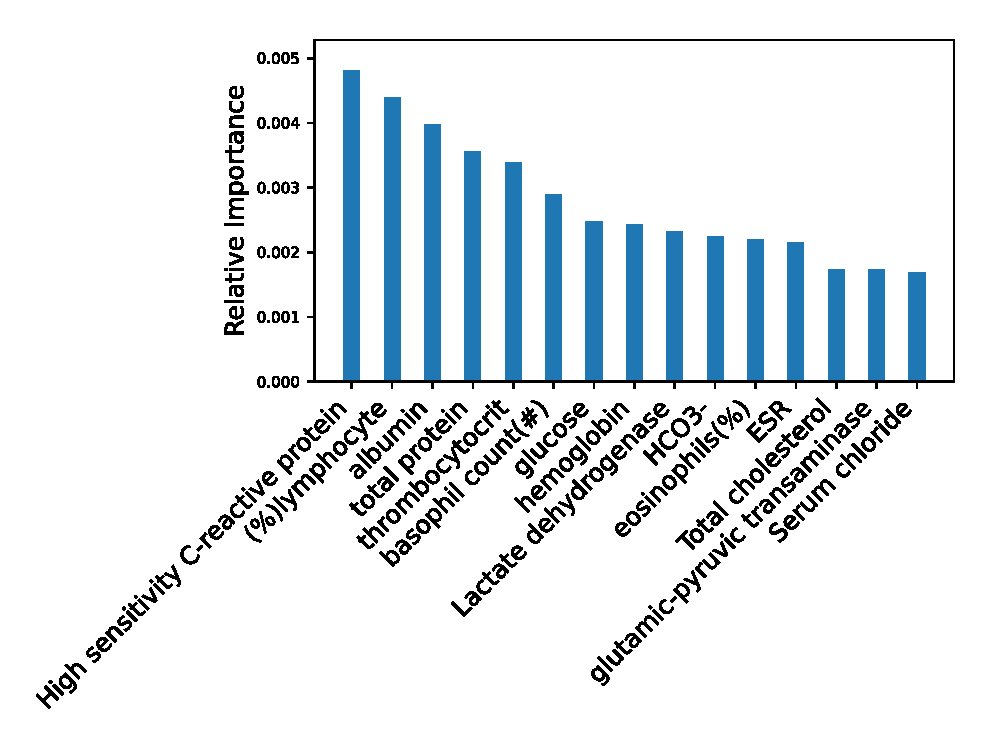
\includegraphics[width=1.0\linewidth]{figures/identified-features.eps}
    \caption{Top 15 important biomarkers identified by the proposed method.} \label{fig: identified-features}
\end{figure}
The identified biomarkers have been shown in the literature to be related to the mortality of COVID-19 patient. For example, lactic dehydrogenase (LDH), lymphocyte and high-sensitivity C-reactive protein (hs-CRP) are the top 3 biomarkers relevant with the mortality of COVID-19 patients, identified by the XGBoost model \cite{yan2020interpretable} and previous medical researches~\cite{kishaba2014staging,ridker2008rosuvastatin,wang2020clinical}. % 11, 12, 16 cited.
To be specific, the increase of LDH indicates tissue or cell destruction and this is the strong sign of tissue or cell damage~\cite{yan2020interpretable}. The activity of idiopathic pulmonary fibrosis can be detected by Serum LDH~\cite{kishaba2014staging}. The hs-CRP is the risk factor for the continuous inflammation~\cite{bajwa2009plasma} and poor prognosis in acute respiratory distress syndrome~\cite{kishaba2014staging,sharma2016aetiology}. The lymphocyte is the common risk factor of COVID-19 patients~\cite{chan2020familial}, and lymphocyte has relation with the decrease in CD4 and CD8 T cells~\cite{liu2020longitudinal}.
Albumin have been found to be independently associated with mortality, at the Cox regression analysis~\cite{violi2020albumin}. The basophil count is known to be the risk factor of mortality and organ injury in COVID-19 patients~\cite{li2020immune}. The biomarkers identified by our model are in nice accordance with the previous studies, and provide the substantial evidence that our approach can identify the features associated with the prediction target.
% Pure LSTM

% The experimental result in \ref{tab: experimetal results} shows 
% It is validation accuracy on test set, not a training set. Output layer of predictor uses sigmoid activation function, and round up the output to generate binary class.

% \subsection{Reconstruction}
% Loss value changes by whether label is given or not, but loss converges stably. : convergency graph.

%% Low standard devation and large test set -> The prediction is stable and robust.

%%% COVID-19 risk factors previous studies.
%% Neutrophil-to-lymphocyte : Neutrophil-to-lymphocyte ratio as an independent risk factor for mortality in hospitalized patients with COVID-19, Yuwei Liu.